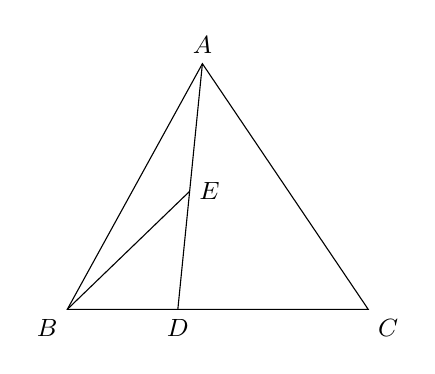
\begin{tikzpicture}[scale=.78, every node/.style={font=\small}]
  \coordinate (A) at (2.20,4); \coordinate (B) at (0,0);
  \coordinate (C) at (4.90,0); \coordinate (D) at (1.80,0);
  \coordinate (E) at (1.99,1.92);
  \draw (A)--(B)--(C)--cycle;
  \draw (A)--(D) (B)--(E);
  \node[above] at (A) {$A$};
  \node[below left] at (B) {$B$};
  \node[below right] at (C) {$C$};
  \node[below] at (D) {$D$};
  \node[right] at (E) {$E$};
\end{tikzpicture}
